\section{From Candidates to Program}


    \critic{red}{Write a better introduction}

    \subsection{Addressing programs with Conditionals}

        We first consider programs with conditionals. 
        The following two properties holds for any candidates of programs having conditional branching. 
        \begin{property}{Candidates of Programs with Conditionals}
            \label{CondB1}
            Let $B1$ be the sets of events based on a branch of a conditional in a program $P$. 
            Let $C$ be any Candidate of $P$ and consider $k$ to be a representative event outside the conditional branch. 
            Then $b1 \in B1$ if and only if:
            \begin{align*}
                \exists C \ \text{s.t.} b1 \notin C  
            \end{align*}
            There exists a candidate of the program such that events from the branch cannot be part of it\footnotemark. 
        \end{property}

        \footnotetext{While the property for 1 branch may not always hold (it can be the case that the branch is always taken in any execution) we are defining it for any program. So we assume that every conditional can either be true or false in a program, not just one of them.}

        The above property is general for conditionals, whether it is an ``if-then" (1-branch) clause or ``if-then-else" (2-branch) clause. 
        The latter however, has another property which we define below:
        \begin{property}{Candidates of Programs with Conditionals (2-branch)}
            \label{CondB2}
            Let $B1,B2$ be two sets of events based on each branch of a conditional in a program $P$. 
            Let $C$ be any Candidate of $P$. 
            Then $b1 \in B1 \ \wedge \ b2 \in B2$ if and only if:
            \begin{align*}
                \nexists C \ \text{s.t.} \ b1 \in C \ \wedge \ b2 \in C \\ 
            \end{align*}
            There cannot exist any candidate of the program such that events from both sets can be part of it\footnotemark. 
        \end{property}

        \footnotetext{Note that here we consider every statement in the program unique. So a program like ``if $(c)$ then {$x=1;$} else {$x=1;$}", both the writes to $x$ are unique.}

        Figure~\ref{reord:conditionals} summarizes the two forms of conditionals we can have in any program. 
        \begin{figure}[H]
            \centering 
            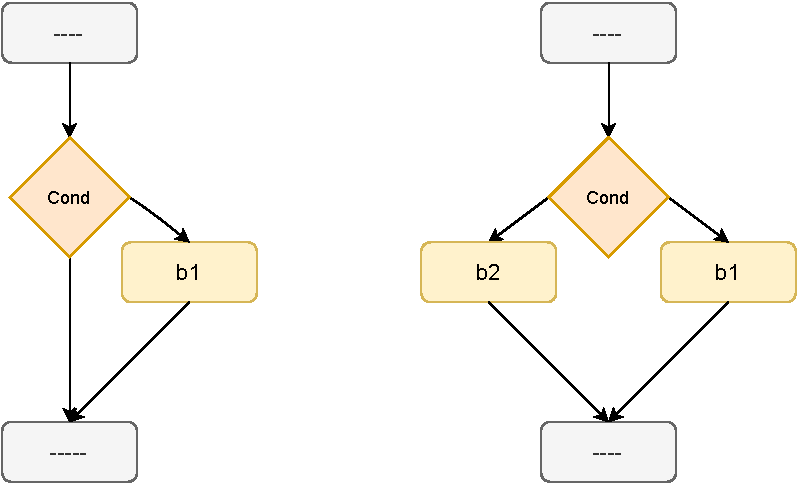
\includegraphics[scale=0.7]{4.InstructionReordering/5.ValidReorderingProgram/Conditionals2Form.pdf}
            \caption{Two forms of conditionals.}
            \label{reord:conditionals}
        \end{figure}


        We use the above two properties to state the following lemma 
        \begin{lemma}
            \label{CondBranchLemma}
            Reordering an statement $e$ inside a conditional to outside a conditional violates Property \ref{CondB1} and Property \ref{CondB2}
        \end{lemma}

        \begin{proof}
            The proof is trivial. 
            By removing a statement outside of a conditional branch, we can get a candidate of a program that would violate both properties. 
        \end{proof}

        The above proof also lets us infer that on reordering an event outside a conditional, there are Candidates that exist with a new event belonging to it. 
        We use this insight to state the following corollary for reordering under conditionals. 
        \begin{corollary}
            \label{ReordCond}
            Consider a program $P$ with conditional branches and its candidates $C_1, C_2, ... , C_n$ in which events $e$ and $d$ present in all of them with $\reln{e}{ao}{d}$. 
            Consider the set of corresponding candidates $C'_1, C'_2, ... , C'_n$ after reordering $e$ and $d$ and its corresponding program $P'$. 
            If the following two conditions hold:
            \begin{gather*}
                Reord(e,d) \ \wedge \ 
                ( \forall C_{i \in [1,n]}, \forall k \in C_i \ \text{s.t.} \ \reln{e}{ao}{k} \wedge \reln{k}{ao}{d}, \    
                Reord(e,k) \wedge Reord(k,d) ). \\
                \nexists C \ s.t. \ 
                    (
                        (e \in C \ \wedge \ d \notin C) \ \vee \ 
                        (e \notin C \ \wedge \ d \in C)
                    ). 
            \end{gather*}
            then the set of observable behaviors of $P'$ is a subset of that of $P$. 
        \end{corollary}

        \begin{proof}

            We prove the second condition first. 
            Assume the second condition does not hold. 
            Then we would have
            \begin{align*}
                \exists C \in P \ s.t. \ 
                (
                    (e \in C \ \wedge \ d \notin C) \ \vee \ 
                    (e \notin C \ \wedge \ d \in C)
                ).
            \end{align*}
            
            By Property \ref{CondB1}, $e$ or $d$ must belong to a conditional branch. 
            If $e$ and $d$ are in different branches of same conditional, then by Property \ref{CondB2} there wouldn't exist any candidate $C$ in $P$ where we could reorder $e$ and $d$. 
            If $e$ and $d$ are of the same conditional branch, and neither one of them belong in any conditional branch nested within, then our above assumption does not hold (simple sequential property of conditional branches).
            
            For the other cases, without loss of generality, let us suppose the first condition holds, i.e. 
            \begin{align*}
                \exists C \in P \ s.t. \ 
                (e \in C \ \wedge \ d \notin C).
            \end{align*}

            The cases for the above can be summarized in the Figure~\ref{reord:cond_branch_cases}: 
            \begin{figure}[H]
                \label{CondCases}
                \centering 
                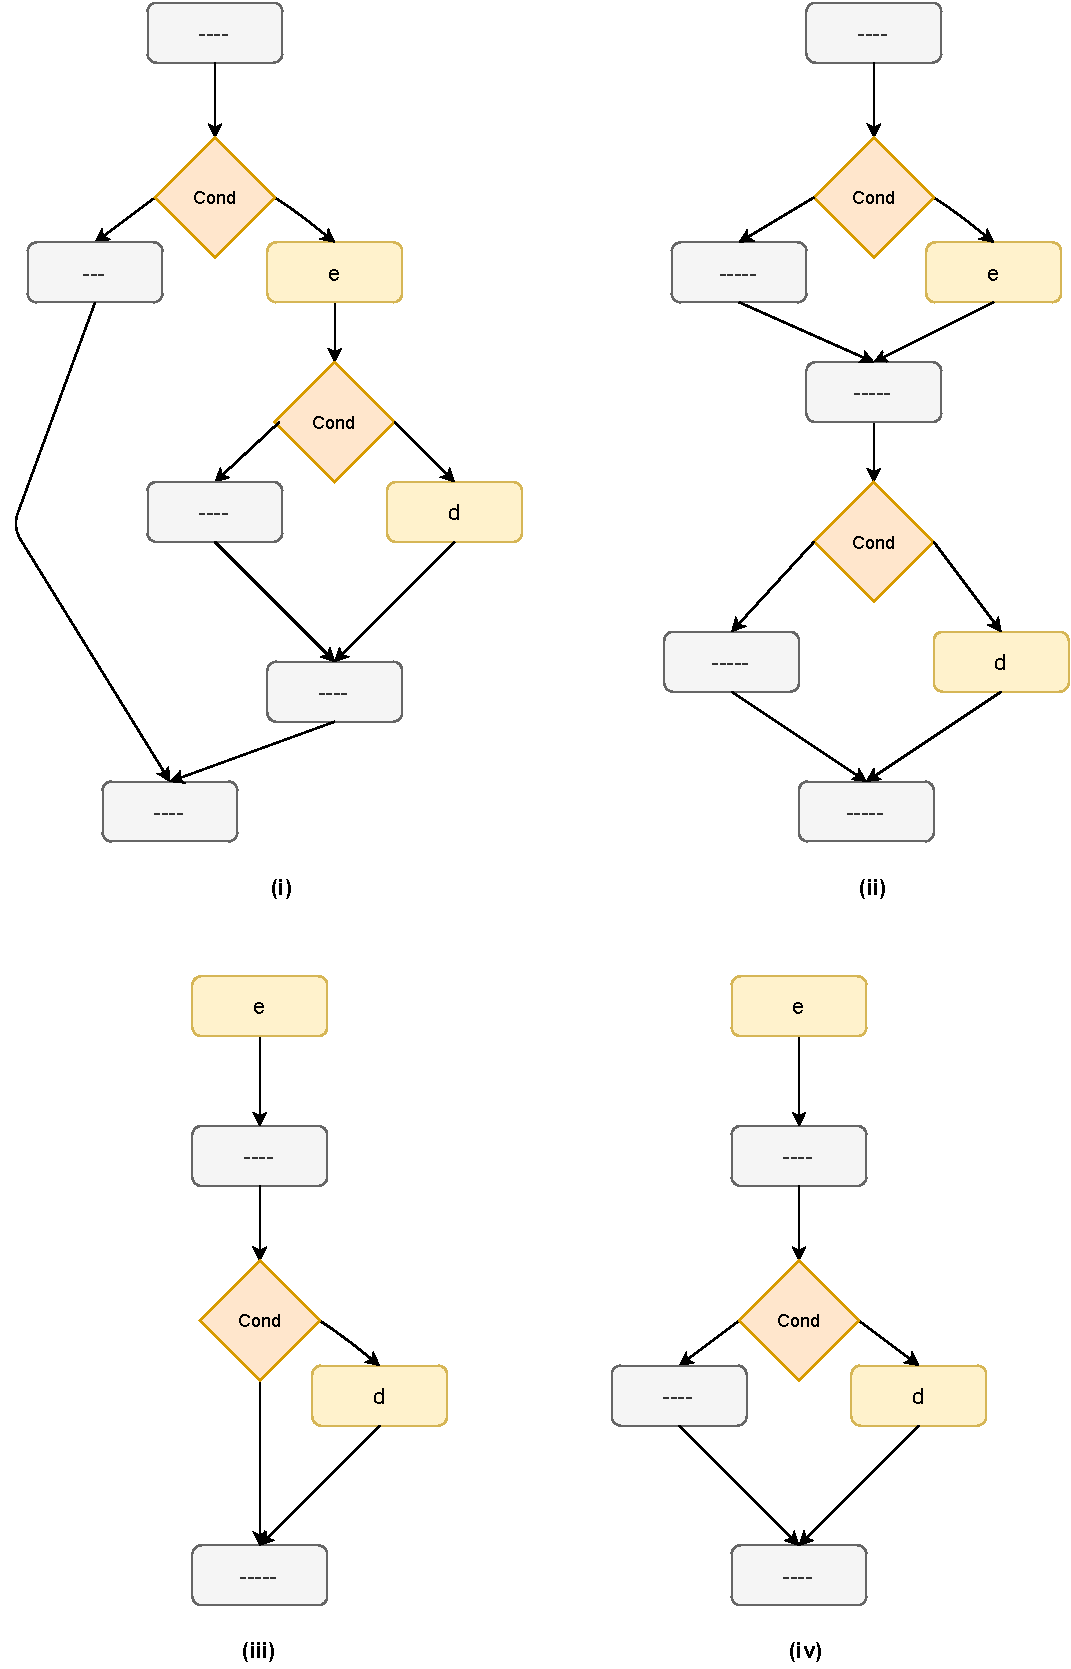
\includegraphics[scale=0.6]{4.InstructionReordering/5.ValidReorderingProgram/ConditionalCases.pdf}
                \caption{Four base cases where $e$ or $d$ are part of some conditional branch.}
                \label{reord:cond_branch_cases}
            \end{figure}

            For cases (i) and (ii), by Lemma \ref{CondBranchLemma}, a new Candidate with event $e$ or $d$ exists without their respective conditional branches being taken.
            For cases (iii) and (iv), by Lemma \ref{CondBranchLemma}, a new Candidate with event $d$ exists without its respective conditional branch being taken.
            Irrespective of $e$ or $d$ being a read or a write, there could be a new $\stck{_{rf}}$ relation be formed with some event $k$ in the Candidate. Thus, we have a new observable behavior\footnotemark. 

            Hence, by contradiction, the second condition must hold.
            
            \footnotetext{Note that this argument is purely in terms of the execution graphs. The new event can possibly have a new reads-from relation established with some event in the graph itself. Since this new node did not exist in the graph before, and since every node in the graph is considered unique, we can infer that a new observable behavior is introduced. Analyzing which such execution graphs are equivalent, would imply drawing equivalence between two different reads-from relations. This could be done as a whole by addressing redundancy introduction optimization. This is not within the scope of the thesis.}

            The first condition holds trivially as it corresponds to Corollary \ref{CorollReord} for each candidate $C_{i\in[1,n]}$. 
            By property of union of sets, we can infer that the set of Observable Behaviors of $P'$ is a subset of that of $P$.

        \end{proof}

  
%------------------------------------------------------------------------------------------------------------------------------------------
    

    \subsection{Addressing Programs with Loops}
    
        Similar to reordering, for the sake of elimination, we consider programs with just one loop. 
        
        %Corollary proof for read elimination within a loop
        We first consider the simpler case of read elimination within a loop. 
        Eliminating such a read at a program level would imply in every candidate $C^i$ where $i$ denotes the number of iterations, the read $R$ within the loop can be eliminated.
        
        By Thereom \ref{ReadElim}, we only need the read $R$ to have the type $uo$ to perform such an elimination.
        Thus we can eliminate for each iteration of the loop our intended read. 
        By transitive property of subsets, the resultant candidate will have observable behaviors as a subset of the original. 
        Doing this for all valid canddiates extends to program level.

        Next we consider the case of eliminating writes within a loop. 
        Eliminating such a write at a program level would imply in every candidate $C^i$ where $i$ denotes the number of iterations, the read $W$ within the loop can be eliminated.
        For this we state the following corollary.
        \begin{corollary}
            Consider a program $P$ having one loop with $K$ representing the set of events within the loop. Consider appropriately candidates $C^1, C^2, ... , C^n$ each of which contain events $e$ and $d$ such that:
            \begin{align*}
                \event{e}{W} \ \wedge \ \event{d}{W} \ \wedge \ \reln{e}{ao}{d} \ \wedge \ \Re(e)\!=\!\Re(d) \ \wedge \ \et{e}{uo}
            \end{align*}
            Consider program $P'$ after eliminating $e$. 
            If
            \begin{align*}
                  \forall C^{i \ in [1,n]} \ \forall k \in C^i \ \text{s.t.} \ \reln{e}{ao}{k} \wedge \reln{k}{ao}{d}, \ Reord(e,k). \\ 
                  \nexists C \in P \ \text{s.t.} \event{e}{C} \ \wedge \  d \notin C.
            \end{align*}
            then the observable behaviors of $P'$ is a subset of that of $P$. 
        \end{corollary}


        \begin{proof}
            
            We need to show that in each iteration of some $C^i$ the write $e$ can be eliminated. 
            For this, we need to have some write $d$ that can exist in all candidates where $e$ can exist. 
            This condition corresponds to Corollary \ref{WriteElimCond}, which handles the case of conditonals too. 
            The set of conditions for observable behaviors of the resultant program to be a subset is Corollary \ref{CorolWriteElim} being applied successively for each candidate $C^i$ and all its iterations where $e$ and $d$ exist. 
            By transitive property of subsets, we can infer that the resultant candidate $C'^i$ has observable behaviors as a subset of original $C^i$. 
            Doing this for all valid canddiates extends to program level by property of union of sets and subset relations\footnotemark.
    
            \footnotetext{One might ideally think based on Theorem \ref{WriteElim} that we could relax the constraint on the existence of $d$ as there is another write $e$ that would exist in the subsequent loop. This however, would rely on the fact that the last iteration of the loop in any execution of the program is guaranteed to have such an event $d$. This is not possible to ascertain as we do not have any information about the number of iterations of the loop. It may also be the case that the loop may never end.}
                
        \end{proof}
         

        \subsubsection{Loop Invariant Code motion}  

            In the previous chapter, we showed that loop invariant code motion cannot be validated by just reordering at the Candidate level. 
            This was because reordering was insufficient to generate the resultant candidate from the original. 
            Because a loop can have any number of iterations, we may have equal number of reads/writes as the iterations. 
            The crux is that now we have proven when elimination is valid under the relaxed memory model. 
            This in conjunction with reordering helps us determine the conditions under which loop invariant code motion can be valid.
            For each case, we use the same property that the resultant candidate execution, and hence candidate to program, the observable behaviors are a subset. 

            We first consider the case of reordering a Read outside a loop. There are two subcases for this, viz. one reordering the read before and one after the loop. 
            \begin{corollary}
    \label{LoopInvCodeMotRead1}
    Consider $K$ to be the set of events within a loop in program $P$. 
    Consider $e$ to be a read within the loop, not being a conditional check. 
    Consider program $P'$ with event $e$ agent ordered before the loop. 
    If
    \begin{gather}
        \et{e}{uo}. \label{licmr1:eq1}\\
        \forall k\!\neq\!e \in K, \ Reord(k, e). \label{licmr1:eq2}\\ 
        \nexists C^i \in P \ \text{s.t.} \ e^{j \leq i} \notin C.  \label{licmr1:eq3}                    
    \end{gather}
    then the set of observable behaviors of $P'$ is a subset of $P$.
\end{corollary}

\begin{proof}

    We first consider the programs with just one iteration of the loop; Candidates of the form $C^1$, having just $e^1$. 
    We need to ensure that the resultant candidates $C^{1}'$ such that 
    \begin{align*}
        \forall k \in K, \ \reln{e}{ao}{k}.
    \end{align*}  
    has observable behaviors as a subset of $C^1$

    For every $k \in K$ such that $\reln{k}{ao}{e}$ we need them to be reorderable with respect to $e$ to bring it outside the loop.
    Using Condition \ref{licmr1:eq2}, we have from Corollary \ref{CorollCodeMotion1} that $C^{1}'$ has observable behaviors as a subset of $C^1$.
    To extend this to the program level with one iteration, we also need that $e$ should not be in any conditional branch.
    Using Condition \ref{licmr1:eq3}, we have from Prop \ref{CondB1} that $e$ is not part of any conditional branch.
    Thus, from Corollary \ref{ReordCond}, we can infer that the transformed program has observable behaviors a subset of the original.  
    
    Next, we consider the program with more than one iteration of the loop. 
    We prove this case using induction on the number of reads $e$ that exist due to multiple iterations of the loop. 
    \begin{itemize}

        \item Base case : number of $e$ = 2
    
        This case corresponds to candidates of the form $C^2$, thus giving us possibly two reads $e^1$ and $e^2$.
        We need candidate $C^2'$ with just one such event $e$, such that:
        \begin{align*}
            \forall k \in K, \ \reln{e}{ao}{k}.
        \end{align*}
        We first want tp reorder both the reads $e^1$, $e^2$ to be outside the loop, naming it Candidate $C^{2}''$.
        Using Condition \ref{licmr1:eq2}, by Corollary \ref{CorollCodeMotion1}, we can infer that $C^{2}''$ has observable behaviors as a subset of $C^2$. 
        From Condition \ref{licmr1:eq1}, by Theorem \ref{ReadElim}, we can eliminate either $e^1$ or $e^2$, thus resulting in $C^2'$ whose observable behaviors is a subset of $C^{2}''$.
        By transitive property of subsets we can infer that $C^2'$ has observable behaviors as a subset of $C^2$.
        %Using Condition \ref{licmr1:eq3}, we can infer that neither $e^1$ nor $e^2$ is part of a conditional.
        %Thus, by Corollary \ref{ReordCond}, we can infer that the transformed program has observable behaviors as a subset of the original.
        
        \item Inductive case : number of $e$ = $n$

        Assume that for all such candidates with $n$ iterations of the loop, the observable behaviors of $C^{n}'$ is a subset of $C^n$.

        We now prove using this that it can also hold for number $e$ as $n + 1$. 
        This case corresponds to candidates of the form $C^{n+1}$, thus giving us $n+1$ reads $e^1, e^2,...,e^{n+1}$.
        From Condition \ref{licmr1:eq2}, we can infer 
        \begin{align*}
            \forall k \ \text{s.t.} \ \reln{e^n}{ao}{k} \wedge \reln{k}{ao}{e^{n+1}}, \ Reord(k,e^{n+1}).
        \end{align*}
        By Corollary \ref{CorollCodeMotion1}, we can infer that $C''^{n+1}$ with $cons(e^n, e^{n+1})$ has observable behaviors as a subset of $C^{n+1}$. 
        From Condition \ref{licmr1:eq1}, by Theorem \ref{ReadElim}, we can eliminate $e^{n+1}$, thus giving us candidate of the form $C^n$ whose observable behaviors is a subset of $C^{n+1}''$.

        From our inductive assumption, we can then conclude that $C^{n+1}'$ has observable behaviors as a subset of $C^n$. 
        By transitive property of subsets, we can infer that $C^{n+1}'$ has observable behaviors as a subset of $C^{n+1}$.

    \end{itemize}

    From Condition \ref{licmr1:eq3}, by Corollary \ref{ReordCond}, we can infer that the observable behaviors of $P'$ is a subset of $P$.
    
\end{proof}

%-----------------------------------------------------------------------------------------------------------------------------------------

\begin{corollary}
    \label{LoopInvCodeMotRead2}
    Consider $K$ to be the set of events within a loop in program $P$. 
    Consider $e$ to be a read within the loop, not being a conditional check. 
    Consider program $P'$ with event $e$ agent ordered after the loop. 
    If
    \begin{gather}
        \et{e}{uo}. \label{licmr2:eq1}\\
        \forall k \neq e \in K, \ Reord(e, k). \label{licmr2:eq2}\\ 
        \nexists C^i \in P \ \text{s.t.} \ e^{j<=i} \notin C.  \label{licmr2:eq3}                    
    \end{gather}
    then the set of observable behaviors of $P'$ is a subset of $P$.
\end{corollary}

\begin{proof}

    We first consider the program with just one iteration. 
    Hence for Candidate $C^1$, we have just $e^1$. 
    We need to ensure that the resultant candidate $C^{1}'$ such that 
    \begin{align*}
        \forall k \in K, \ \reln{k}{ao}{e}.
    \end{align*}  
    has observable behaviors as a subset of $C^1$

    For every $k \in K$ such that $\reln{e}{ao}{k}$ we need them to be reorderable with respect to $e$ to bring it outside the loop.
    Using Condition \ref{licmr1:eq2}, we have from Corollary \ref{CorollCodeMotion1} that $C^{1}'$ has observable behaviors as a subset of $C^1$.
    To extend this to the program level with one iteration, we also need that $e$ should not be in any conditional branch.
    Using Condition \ref{licmr1:eq3}, we have from Prop \ref{CondB1} that $e$ is not part of any conditional branch.
    Thus, from Corollary \ref{ReordCond}, we can infer that the transformed program has observable behaviors a subset of the original.  
    
    Next, we consider the program with more than one iteration of the loop. 
    We prove this case using induction on the number of reads $e$ that exist due to multiple iterations of the loop. 
    \begin{itemize}
        
        \item Base case : number of $e$ = 2
    
        This case corresponds to candidates of the form $C^2$, thus giving us possibly two reads $e^1$ and $e^2$.
        We need candidate $C'^2$ with just one such event $e$, such that:
        \begin{align*}
            \forall k \in K, \ \reln{k}{ao}{e}.
        \end{align*} 
        We first reorder both the reads $e^1$, $e^2$ to be outside the loop, naming it Candidate $C''^2$.
        Because we have Condition \ref{licmr2:eq2}, by Corollary \ref{CorollCodeMotion1}, we can infer that $C''^2$ has observable behaviors as a subset of $C^2$.
        To go from $C^{2}''$ to $C^2'$, note that in $C^{2}''$ we have $cons(e^1, e^2)$ after reordering them. 
        From Condition \ref{licmr2:eq1}, by Theorem \ref{ReadElim}, we can eliminate either $e^1$ or $e^2$, thus resulting in $C^2'$ whose observable behaviors is a subset of $C^{2}''$.
        
        By transitive property of subsets we can infer that $C^2'$ has observable behaviors as a subset of $C^2$.
        
        \item Inductive case : number of $e$ = n

        Assume that for all such candidates with $n$ iterations of the loop, the observable behaviors of $C'^n$ is a subset of $C^n$.

        We now prove using this that it can also hold for number $e$ as $n + 1$. 
        This case corresponds to candidates of the form $C^{n+1}$, thus giving us $n+1$ reads $e^1, e^2,...,e^{n+1}$.
        From Condition \ref{licmr1:eq2}, we can infer
        \begin{align*}
            \forall k \ \text{s.t.} \ \reln{e^n}{ao}{k} \wedge \reln{k}{ao}{e^{n+1}}, \ Reord(e^{n}, k)
        \end{align*}
        By Corollary \ref{CorollCodeMotion1}, we can infer that $C''^{n+1}$ with $cons(e^n, e^{n+1})$ has observable behaviors as a subset of $C^{n+1}$. 
        From Condition \ref{licmr2:eq1}, by Theorem \ref{ReadElim}, we can eliminate $e^{n+1}$, thus giving us candidate of the form $C^n$ whose observable behaviors is a subset of $C^{n+1}''$.
        From our inductive assumption, we can then conclude that $C^{n+1}'$ has observable behaviors as a subset of $C^n$. 
        By transitive property of subsets, we can infer that $C^{n+1}'$ has observable behaviors as a subset of $C^{n+1}$.

    \end{itemize}

    From Condition \ref{licmr2:eq3}, by Corollary \ref{ReordCond}, we can infer that the observable behaviors of $P'$ is a subset of $P$.
    
\end{proof}            

            Now we consider the case of reordering a write outside a loop, similar two sub-cases as for reads.           
            \begin{corollary}
    \label{LoopInvCodeMotWrite1}
    Consider $K$ to be the set of events within a loop in program $P$. 
    Consider $e$ to be a write within the loop. 
    Consider program $P'$ with event $e$ agent ordered before the loop. 
    If
    \begin{gather}
        \et{e}{uo}. \label{licmw1:eq1}\\
        \forall k \neq e \in K, \ Reord(k, e). \label{licmw1:eq2} \\ 
        \nexists C^i \in P \ \text{s.t.} \ e^{j<=i} \notin C.  \label{licmw1:eq3}                    
    \end{gather}
    then the set of observable behaviors of $P'$ is a subset of $P$.

\end{corollary}             

\begin{proof}


    We first consider the program with just one iteration. Hence for Candidate $C^1$, we have just $e^1$. 
    We need to ensure that the resultant candidate $C'^1$ such that 
    \begin{align*}
        \forall k \in K, \ \reln{e}{ao}{k}.
    \end{align*}  
    has observable behaviors as a subset of $C^1$

    For every $k \in K$ such that $\reln{k}{ao}{e}$ we need them to be reorderable with respect to $e$ to bring it outside the loop.
    Using Condition \ref{licmw1:eq2}, we have from Corollary \ref{CorollCodeMotion1} that $C^1'$ has observable behaviors as a subset of $C^1$.
    To extend this to the program level with one iteration, we also need that $e$ should not be in any conditional branch.
    Using Condition \ref{licmw1:eq3}, we have from Prop \ref{CondB1} that $e$ is not part of any conditional branch.
    Thus, from Corollary \ref{ReordCond}, we can infer that the transformed program has observable behaviors a subset of the original.  
    
    Next, we consider the program with more than one iteration of the loop. 
    We prove this case using induction on the number of reads $e$ that exist due to multiple iterations of the loop. 
    \begin{itemize}

        \item Base case : number of $e$ = 2
        This case corresponds to candidates of the form $C^2$, thus giving us two writes eads $e^1$ and $e^2$.
        We need candidate $C^2'$ with just one such event $e$, such that:
        \begin{align*}
            \forall k \in K, \ \reln{k}{ao}{e}.
        \end{align*}  
        We first reorder both the writes $e^1$, $e^2$ to be outside the loop, naming it Candidate $C^2''$.
        Because we have Condition \ref{licmr2:eq2}, by Corollary \ref{CorollCodeMotion1}, we can infer that $C''^2$ has observable behaviors as a subset of $C^2$.
        To go from $C^2''$ to $C^2'$, note that in $C^2''$ we have $cons(e^1, e^2)$ after reordering them. 
        From Condition \ref{licmr2:eq1}, by Theorem \ref{WriteElim}, we can eliminate $e^1$, thus resulting in $C'^2$ whose observable behaviors is a subset of $C''^2$\footnotemark.

        \footnotetext{Note that here, it is only safe to eliminate the first write ($e^1$) in contrast to having the choice to eliminate either $e^1$ or $e^2$ when both are reads.}
        
        By transitive property of subsets we can infer that $C^2'$ has observable behaviors as a subset of $C^2$.
        
        \item Inductive case : number of $e$ = n

        Assume that for all such candidates with $n$ iterations of the loop, the observable behaviors of $C^n'$ is a subset of $C^n$.

        We now prove using this that it can also hold for number $e$ as $n + 1$. 
        This case corresponds to candidates of the form $C^{n+1}$, thus giving us $n+1$ reads $e^1, e^2,...,e^{n+1}$.
        From Condition \ref{licmw1:eq2} we can infer 
        \begin{align*}
            \forall k \ \text{s.t.} \ \reln{e^n}{ao}{k} \wedge \reln{k}{ao}{e^{n+1}}, \ Reord(k,e^{n+1}).
        \end{align*}
        By Corollary \ref{CorollCodeMotion1}, we can infer that $C^{n+1}''$ with $cons(e^n, e^{n+1})$ has observable behaviors as a subset of $C^{n+1}$. 
        From Condition \ref{licmw1:eq1}, by Theorem \ref{WriteElim}, we can eliminate $e^{n}$, thus giving us candidate of the form $C^n$ whose observable behaviors is a subset of $C^{n+1}''$.
        From our inductive assumption, we can then conclude that $C^{n+1}'$ has observable behaviors as a subset of $C^n$. 
        By transitive property of subsets, we can infer that $C^{n+1}'$ has observable behaviors as a subset of $C^{n+1}$.

    \end{itemize}

    From Condition \ref{licmw1:eq3}, by Corollary \ref{ReordCond}, we can infer that the observable behaviors of $P'$ is a subset of $P$.

\end{proof}


\begin{corollary}
    \label{LoopInvCodeMotWrite2}
    Consider $K$ to be the set of events within a loop in program $P$. 
    Consider $e$ to be a write within the loop. 
    Consider program $P'$ with event $e$ agent ordered before the loop. 
    If
    \begin{gather*}
        \et{e}{uo}. \label{licmw2:eq1}\\
        \forall k \neq e \in K, \ Reord(e, k). \label{licmw2:eq2}\\ 
        \nexists C^i \in P \ \text{s.t.} \ e^{j<=i} \notin C.  \label{licmw2:eq3}                    
    \end{gather*}
    then the set of observable behaviors of $P'$ is a subset of $P$.

\end{corollary}             

\begin{proof}

    We first consider the program with just one iteration. 
    Hence for Candidate $C^1$, we have just $e^1$. 
    We need to ensure that the resultant candidate $C'^1$ such that 
    \begin{align*}
        \forall k \in K, \ \reln{k}{ao}{e}.
    \end{align*}  
    has observable behaviors as a subset of $C^1$

    For every $k \in K$ such that $\reln{e}{ao}{k}$ we need them to be reorderable with respect to $e$ to bring it outside the loop.
    Using Condition \ref{licmw2:eq2}, we have from Corollary \ref{CorollCodeMotion1} that $C^1'$ has observable behaviors as a subset of $C^1$.
    To extend this to the program level with one iteration, we also need that $e$ should not be in any conditional branch.
    Using Condition \ref{licmw2:eq3}, we have from Prop \ref{CondB1} that $e$ is not part of any conditional branch.
    Thus, from Corollary \ref{ReordCond}, we can infer that the transformed program has observable behaviors a subset of the original.   
    
    Next, we consider the program with more than one iteration of the loop. 
    We prove this case using induction on the number of reads $e$ that exist due to multiple iterations of the loop. 

    \begin{itemize}

        \item Base case : number of $e$ = 2
        This case corresponds to candidates of the form $C^2$, thus giving us two writes $e^1$ and $e^2$.
        We need candidate $C^2'$ with just one such event $e$, such that:
        \begin{align*}
            \forall k \in K, \ \reln{k}{ao}{e}.
        \end{align*}  
        We also have from property of loops that $\reln{e^1}{ao}{e^2}$.
        Having Condition \ref{licmw2:eq1}, \ref{licmw2:eq2}, by Corollary \ref{CorolWriteElim}, we can eliminate $e^1$, giving us $C^2''$ whose observable behaviors as a subset of $C^2$.  
        From Corollary \ref{CorollCodeMotion2}, we can reorder $e^2$ outside the loop thus giving us $C^2'$ whose observable behaviors as a subset of $C^2''$.
        
        By transitive property of subsets we can infer that $C^2'$ has observable behaviors as a subset of $C^2$.
        
        \item Inductive case : number of $e$ = n

        Assume that for all such candidates with $n$ iterations of the loop, the observable behaviors of $C^n'$ is a subset of $C^n$.

        We now prove using this that it can also hold for number $e$ as $n + 1$. 
        This case corresponds to candidates of the form $C^{n+1}$, thus giving us $n+1$ reads $e^1, e^2,...,e^{n+1}$.
        From Condition \ref{licmw2:eq2}, we can infer 
        \begin{align*}
            \forall k \ \text{s.t.} \ \reln{e^n}{ao}{k} \wedge \reln{k}{ao}{e^{n+1}}, \ Reord(e^{n}, k).
        \end{align*}
        Having Condition \ref{licmw2:eq1}, by Corollary \ref{CorolWriteElim}, we can eliminate $e^{n}$, thus giving us candidate $C^{n}$ whose observable behaviors are a subset of $C^{n+1}$

        From our inductive assumption, we can then conclude that $C^{n+1}'$ has observable behaviors as a subset of $C^n$. 
        By transitive property of subsets, we can infer that $C^{n+1}'$ has observable behaviors as a subset of $C^{n+1}$.

    \end{itemize}
    
    From Condition \ref{licmw2:eq3}, by Corollary \ref{ReordCond} and \ref{WriteElimCond}, we can infer that the observable behaviors of $P'$ is a subset of $P$.

\end{proof}


            

            \paragraph{Reordering two events accross loops} 
            
            The above corollaries are defined for programs with one loop. 
            However, they are valid for whenever loop invariant code motion is just involving removing an event outside one loop. 
            In practice programs can have multiple loops, even those nested within each other and the compiler is free to reorder events accross nesting as well as from one loop to another.
            We cannot prove when we can reorder events accross two different loops or reordering events to be within a loop.
            At the Candidate level, this would imply reordering, elimination as well as \textbf{introduction} of events. 
            Hence, this would require a proof of redundancy introduction right from the candidate execution level and then be extended to candidates and then to programs. 
            This is beyond the scope of this thesis. We consider this as a part of future work. 